%=========================================================
\chapter{Planeación del Tiempo}	
\label{cap:tiempo}

	Este capítulo presenta el desglose de la planeación del tiempo del proyecto, contiene la lista de actividades, entregables y esfuerzo requerido para el proyecto, así como las metodologías a utilizar.

%---------------------------------------------------------
\section{Diagrama de Gantt}

\begin{figure}[htbp!]
	\begin{center}
		\fbox{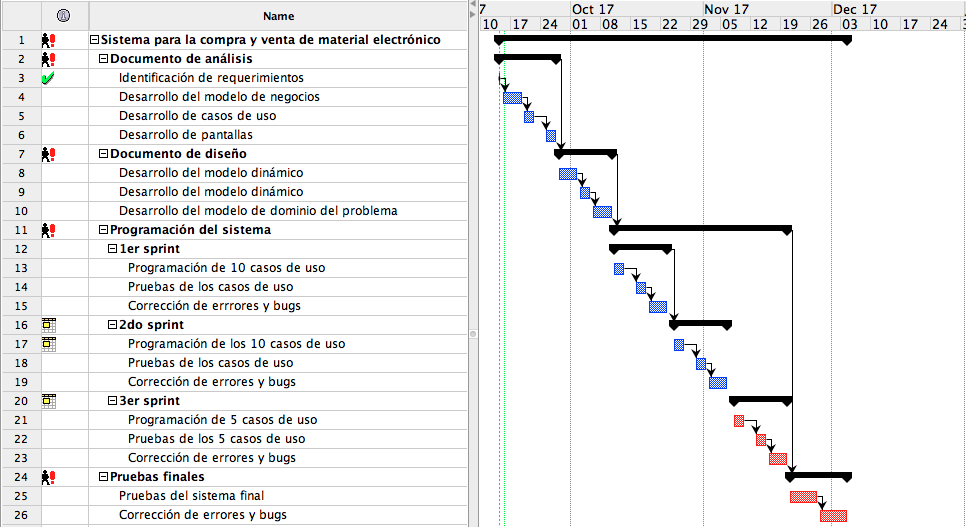
\includegraphics[width=.8\textwidth]{images/plan}}
		\caption{Plan de trabajo del proyecto}
		\label{fig:plan}
	\end{center}
\end{figure}

%---------------------------------------------------------
\section{Entregables}

Los entregables que se tendrán durante el desarrollo del proyecto son los siguientes:

\begin{enumerate}
	\item E2 - Documento de análisis: Miércoles 27 de Septiembre de 2017.
	\item E3 - Documento de diseño: Miércoles 11 de Octubre de 2017.
	\item E4 - Programación de 10 casos de uso y pruebas: Miércoles 25 de Octubre de 2017.
	\item E5 - Programación de 10 casos de uso y pruebas: Miércoles 08 de Nombre de 2017.
	\item E6 - Programación de 5 casos de uso y pruebas: Miércoles 22 de Noviembre de 2017.
	\item E7 - Corrección de errores y sistema final: Miércoles 06 de Diciembre de 2017.
\end{enumerate}

